% Basic setup. Most papers should leave these options alone.
\documentclass[fleqn,usenatbib]{mnras}

% MNRAS is set in Times font. If you don't have this installed (most LaTeX
% installations will be fine) or prefer the old Computer Modern fonts, comment
% out the following line
\usepackage{newtxtext,newtxmath}
% Depending on your LaTeX fonts installation, you might get better results with one of these:
%\usepackage{mathptmx}
%\usepackage{txfonts}

% Use vector fonts, so it zooms properly in on-screen viewing software
% Don't change these lines unless you know what you are doing
\usepackage[T1]{fontenc}

% Allow "Thomas van Noord" and "Simon de Laguarde" and alike to be sorted by "N" and "L" etc. in the bibliography.
% Write the name in the bibliography as "\VAN{Noord}{Van}{van} Noord, Thomas"
\DeclareRobustCommand{\VAN}[3]{#2}
\let\VANthebibliography\thebibliography
\def\thebibliography{\DeclareRobustCommand{\VAN}[3]{##3}\VANthebibliography}


%%%%% AUTHORS - PLACE YOUR OWN PACKAGES HERE %%%%%

% Only include extra packages if you really need them. Avoid using amssymb if newtxmath is enabled, as these packages can cause conflicts. newtxmatch covers the same math symbols while producing a consistent Times New Roman font. Common packages are:
\usepackage{graphicx}	% Including figure files
\usepackage{amsmath}	% Advanced maths commands

%%%%%%%%%%%%%%%%%%%%%%%%%%%%%%%%%%%%%%%%%%%%%%%%%%

%%%%% AUTHORS - PLACE YOUR OWN COMMANDS HERE %%%%%

% Please keep new commands to a minimum, and use \newcommand not \def to avoid
% overwriting existing commands. Example:
%\newcommand{\pcm}{\,cm$^{-2}$}	% per cm-squared

%%%%%%%%%%%%%%%%%%%%%%%%%%%%%%%%%%%%%%%%%%%%%%%%%%

%%%%%%%%%%%%%%%%%%% TITLE PAGE %%%%%%%%%%%%%%%%%%%

% Title of the paper, and the short title which is used in the headers.
% Keep the title short and informative.
\title[Short title, max. 45 characters]{Gravitational wave inference at GPU speed: A \texttt{bilby}-like nested sampler within \texttt{blackjax-ns}}

% The list of authors, and the short list which is used in the headers.
% If you need two or more lines of authors, add an extra line using \newauthor
\author[Metha Prathaban et al.]{
Metha Prathaban,$^{1}$\thanks{E-mail: myp23@cam.ac.uk (MP)}
David Yallup,$^{2}$
James Alvey$^{2,3}$
and Will Handley$^{3}$
\\
% List of institutions
$^{1}$University of Cambridge, Cambridge, CB3 0HE, UK\\
$^{2}$\\
$^{3}$
}

% These dates will be filled out by the publisher
\date{Accepted XXX. Received YYY; in original form ZZZ}

% Prints the current year, for the copyright statements etc. To achieve a fixed year, replace the expression with a number. 
\pubyear{\the\year{}}

% Don't change these lines
\begin{document}
\label{firstpage}
\pagerange{\pageref{firstpage}--\pageref{lastpage}}
\maketitle

% Abstract of the paper
\begin{abstract}
This is a simple template for authors to write new MNRAS papers.
The abstract should briefly describe the aims, methods, and main results of the paper.
It should be a single paragraph not more than 250 words (200 words for Letters).
No references should appear in the abstract.
\end{abstract}

% Select between one and six entries from the list of approved keywords.
% Don't make up new ones.
\begin{keywords}
keyword1 -- keyword2 -- keyword3
\end{keywords}

%%%%%%%%%%%%%%%%%%%%%%%%%%%%%%%%%%%%%%%%%%%%%%%%%%

%%%%%%%%%%%%%%%%% BODY OF PAPER %%%%%%%%%%%%%%%%%%

\section{Introduction}



% Bayesian inference serves as the foundation for gravitational wave data analysis, providing a robust framework for computing posterior distributions and evidences.
% Among the various tools available in this domain, nested sampling is particularly popular for its capacity to efficiently perform parameter estimation, model comparison and tension quantification.


% Name popular nested samplers used within established codes such as bilby, lalinference (dynesty, polychord, nessai, cpnest). Both these samplers and codes have been widely tested, but it is known that they are computationally intensive. Whilst still feasible for current experiments, the future brings an entirely different data landscape.

% Compare and contrast current and future data. Talk about scaling of nested sampling in particular, and how all these factors will make the runtime too large. Cite John Veitch's paper on expected runtime, and Mac's paper on single BNS event. Current traditional methods simply will not scale to this era. Moreover, many of the current established acceleration methods may not scale in accuracy to this era either (cite Paul's paper).

% The two biggest technological advancements driving progress in this area. The first is machine learning, which has been used to accelerate waveform evaluation through ROQ, make general improvements to the sampler (nessai), and accelerate the core nested sampling algorithm in other ways (cite my paper, others). Combining these techniques could result in orders of magnitude improvement if properly leveraged. There are also innovative alternative Bayesian inference methods such as SBI which are posed to address future challenges. 

% The other main technological advancement is the introduction of GPUs, and this presents major opportunities for nested sampling in the 3G era. Introduce parallisation. In (david's paper), he introduced a nested sampler designed to be run on GPUs, making use of the parallelization of GPUs. David's paper demonstrated the accuracy and performance of the sampler. Here, we apply it to gravitational wave problems to show its advantages and opportunities in the 3G era.

The era of gravitational wave (GW) astronomy, initiated by the landmark
detections of the Laser Interferometer Gravitational-Wave Observatory (LIGO) and
Virgo, and now advanced by the global network including KAGRA, has revolutionized
our view of the cosmos~\citep{GW150914, GW170817,GWTC1,GWTC2, GWTC3,GWTC3_pop_analysis,GWTC2_GR,siren}. 
Extracting scientific insights from the faint, transient signals buried in detector noise—from measuring the
masses and spins of binary black holes to performing precision tests of general
relativity—relies critically on the framework of Bayesian inference~\citep{Thrane_2019}. 
This allows for the estimation of posteriors on source parameters
(parameter estimation) and the comparison of competing physical models (model selection).

The process of Bayesian inference in GW astronomy is, however, computationally
demanding. Realistic theoretical models for the GW waveform are complex, and the
stochastic sampling algorithms required to explore the high-dimensional parameter
space can require millions of likelihood evaluations per analysis~\citep{LIGO_guide_signalextraction}.
The community-standard software tools, the inference library \texttt{bilby}~\citep{bilby_paper}
paired with a custom implementation of the nested sampler \texttt{dynesty}~\citep{dynesty}, 
have proven to be a robust and highly effective framework, tuned for the specific needs of GW posteriors.
However, this framework is predominantly executed on central processing units
(CPUs), making individual analyses time-consuming and creating a significant
computational bottleneck. This challenge is set to become acute with the
increased data volumes from future observing runs~\citep{aLIGO, aVirgo, aLVK_prospects} and the advent of
next-generation observatories, such as the Einstein Telescope~\citep{ET_science_case}, which promise
unprecedented sensitivity and detection volumes~\citep{HuAccelerationReview}.

In response to this challenge, the GW community has begun to leverage the immense
parallel processing power of graphics processing units (GPUs). Pioneering work in
this domain, such as the \texttt{jimgw} codebase~\citep{wong2023fastgravitationalwaveparameter}, has successfully
implemented GPU-accelerated Markov Chain Monte Carlo (MCMC) samplers like \texttt{flowMC}~\citep{flowMC}, 
paired with GPU implementations of waveform models provided by the
\texttt{ripple} library~\citep{ripple}. This work has demonstrated that
substantial, order-of-magnitude speedups for GW parameter estimation are
achievable. While these MCMC-based approaches excel at rapidly generating samples
from the posterior for parameter estimation, they do not directly compute the
Bayesian evidence, which remains key for robust model selection.

In this paper, we introduce a GPU-accelerated nested sampling
algorithm for gravitational wave data analysis. Our method
builds upon the trusted `acceptance-walk' sampler used in the
community-standard \texttt{bilby} and \texttt{dynesty} framework.
We leverage the \texttt{blackjax ns} sampler, a recent tool
designed for vectorized execution on GPUs~\citep{yallup2025nested}.
This sampler, part of the \texttt{blackjax} library, is a novel reformulation
of the core nested sampling algorithm for massive parallelization~\citep{cabezas2024blackjax}.

Instead of its default slice sampler, we developed a custom
kernel that implements the `acceptance-walk' method. This
ensures our sampler's logic is almost identical to the
\texttt{bilby} and \texttt{dynesty} implementation, with differences
primarily related to parallelization. This approach offers
\texttt{bilby} users a direct path to GPU-accelerated inference for the most expensive problems in GW astronomy.
They can achieve significant speedups while retaining the same
robust and trusted algorithm at the core of their analyses.

% In this paper, we apply a GPU-accelerated version of the `acceptance-walk' nested sampling algorithm in \texttt{bilby} 
% to gravitational wave data analysis. Nested Sampling is a powerful Bayesian algorithm particularly
% regarded for its ability to robustly calculate the evidence while simultaneously
% producing posterior samples, even for complex, multimodal distributions~\citep{skilling}. 
% We employ the \texttt{blackjax ns} sampler,
% recently developed by Yallup et al.~\citep{yallup2025nested} and implemented within the pre-existing software 
% \texttt{blackjax}~\citep{cabezas2024blackjax}. This sampler is based on a novel reformulation of the 
% nested sampling algorithm that is natively vectorized for highly parallel execution on GPUs. Instead of the default 
% slice sampler implemented in~\cite{yallup2025nested}, we use a custom kernel that implements the `acceptance-walk' 
% sampling method used in the \texttt{bilby} code. When run with this kernel, the \texttt{blackjax ns} sampler is 
% designed to be largely identical to the standard \texttt{bilby} + \texttt{dynesty} sampler, with differences only 
% being related to parallelisation. This enables \texttt{bilby} users to migrate to GPU-accelerated sampling with minimal 
% changes to their existing robust algorithms, whilst offering significant speedups.

% We present the first application and validation of this sampler for the analysis of simulated binary 
% black hole mergers. This work complements the existing suite of GPU-MCMC tools by providing a robust implementation of 
% GPU-accelerated nested sampling in this context, thereby unifying rapid parameter estimation and model selection within 
% a single high-performance computational framework.


\section{Background}

\subsection{Bayesian inference in GW astronomy}
\label{sec:background_bayes}
We provide a brief overview of the core concepts of
Bayesian inference as applied to GW astronomy. For a more
comprehensive treatment, we refer the reader to~\cite{skilling, Thrane_2019, lal, bilby_paper, LIGO_guide_signalextraction}.

The analysis of GW signals is fundamentally a problem of statistical
inference, for which the Bayesian framework is the community standard.
The relationship between data, $d$, and a set of source parameters,
$\theta$, under a specific hypothesis, $H$, is given by Bayes' theorem~\citep{Bayes1763}:

\begin{equation}
    p(\theta|d, H) = \frac{\mathcal{L}(d|\theta, H) \pi(\theta|H)}{Z(d|H)}.
    \label{eq:bayes_theorem}
\end{equation}%
Here, the posterior, $p(\theta|d, H)$, is the probability distribution
of the source parameters conditioned on the observed data. It is
determined by the likelihood, $\mathcal{L}(d|\theta, H)$, which is the
probability of observing the data given a specific realisation of the
model, and the prior, $\pi(\theta|H)$, which encodes initial beliefs
about the parameter distributions.

The denominator is the Bayesian evidence,
\begin{equation}
    Z(d|H) = \int \mathcal{L}(d|\theta, H) \pi(\theta|H) d\theta,
    \label{eq:evidence}
\end{equation}
defined as the likelihood integrated over the entire volume of the
prior parameter space.

There are two pillars of Bayesian inference of particular interest
in GW astronomy. The first, parameter estimation, seeks to infer 
the posterior distribution $p(\theta|d, H)$ of the source parameters of a signal or population of signals.
The second, model selection, evaluates two competing
models, $H_1$ and $H_2$, under a fully Bayesian framework by computing the ratio of
their evidences, known as the Bayes factor, $Z_1 / Z_2$. This enables
principled classification of noise versus true signals, as well as the 
comparison of different waveform models.

In GW astronomy, the high dimensionality of the parameter space and
the computational cost of the likelihood render the direct evaluation
of Eq.~\ref{eq:bayes_theorem} and Eq.~\ref{eq:evidence} intractable~\citep{LIGO_guide_signalextraction}.
Analysis therefore relies on stochastic sampling algorithms to
numerically approximate the posterior and evidence.

\subsection{GPU-accelerated nested sampling}

\label{sec:background_ns_and_gpus}

\subsubsection{The nested sampling algorithm}
\label{sec:background_ns}

Nested Sampling (NS) is a Monte Carlo algorithm designed to solve the
Bayesian inference problem outlined in Sec.~\ref{sec:background_bayes}.
A key strength of the NS algorithm is that it directly computes the
Bayesian evidence, $Z$, while also producing posterior samples as a
natural by-product of its execution~\citep{skilling}.

The algorithm starts by drawing a population of $N$ `live points'
from the prior distribution, $\pi(\theta)$. It then proceeds
iteratively. In each iteration, the live point with the lowest
likelihood value, $\mathcal{L}_{\text{min}}$, is identified. This point
is deleted from the live set and stored. It is then replaced with a
new point, drawn from the prior, but subject to the hard constraint that
its likelihood must exceed that of the deleted point,
i.e., $\mathcal{L}_{\text{new}} > \mathcal{L}_{\text{min}}$. This process
systematically traverses nested shells of increasing likelihood, with
the sequence of discarded points mapping the likelihood landscape.

The primary computational challenge within the NS algorithm is the
efficient generation of a new point from the likelihood-constrained
prior~\citep{NSNature}. The specific method used for this `inner sampling' task is a
critical determinant of the sampler's overall efficiency and robustness.

\subsubsection{GPU architectures for scientific computing}
\label{sec:background_gpus}

The distinct architectures of Central Processing Units (CPUs) and
Graphics Processing Units (GPUs) offer different advantages for
computational tasks. CPUs are comprised of a few powerful cores
optimised for sequential task execution and low latency. In contrast,
GPUs feature a massively parallel architecture, containing thousands of
simpler cores designed for high-throughput computation.

This architecture makes GPUs exceptionally effective for problems that can
be expressed in a Single Instruction, Multiple Data (SIMD) paradigm.
In such problems, the same operation is performed simultaneously across
a large number of data elements, leading to substantial performance
gains over serial execution on a CPU. The primary trade-off is that
algorithms must be explicitly reformulated to expose this parallelism,
as not all computational problems are amenable to vectorization.

\subsubsection{A vectorized formulation of nested sampling}
\label{sec:background_vectorized_ns}

The iterative, one-at-a-time nature of the traditional NS algorithm
is intrinsically serial, making it a poor fit for the parallel
architecture of GPUs. To overcome this limitation, Yallup et al.
recently developed a vectorized formulation of the NS algorithm,
specifically designed for highly parallel execution within the
\texttt{blackjax} framework~\citep{yallup2025nested, cabezas2024blackjax}.

One of the core innovations of this approach is the introduction of batch
processing. Instead of replacing a single live point in each iteration,
the algorithm removes a batch of $k$ points with the lowest likelihoods
simultaneously. The critical step of replacing these points is then
parallelized. The algorithm launches $k$ independent sampling processes
on the GPU, with each process tasked with finding one new point that
satisfies the likelihood constraint, $\mathcal{L} > \mathcal{L}_{\text{min}}$,
where $\mathcal{L}_{\text{min}}$ is now the maximum likelihood of the
discarded batch.

This reformulation transforms the computationally intensive task of
sample generation from a serial challenge into a massively parallel one,
thereby leveraging the architectural strengths of the GPU. While the
original work proposed a specific inner sampling kernel for this task,
the vectorized framework itself is general. It provides a structure
within which any suitable inner sampling method can be deployed in
parallel.


\section{Methods}

\subsection{The inner sampling kernel}
\label{sec:methods_kernel}

Several inner sampling methods are implemented within the
\texttt{bilby} and \texttt{dynesty} framework~\citep{bilby_paper, dynesty}. In this work, we
focus on a GPU-accelerated implementation of the `acceptance-walk'
method, which is a robust and widely used choice for GW analyses.

In the standard CPU-based \texttt{dynesty} implementation, the sampler
generates a new live point by initiating a Markov Chain Monte Carlo
(MCMC) walk from the position of a randomly selected existing live
point. The proposal mechanism for the MCMC walk is based on Differential
Evolution (DE)~\citep{DE, DE2}, which uses the distribution of existing live points to
inform jump proposals. A new candidate point is generated by adding a
scaled vector difference of two other randomly chosen live points to the
current point in the chain. Under the default \texttt{bilby} configuration, 
the scaling factor for this vector is chosen stochastically: with equal probability, 
it is either fixed at 1.0 or drawn from a gamma distribution. This proposed 
point is accepted if it satisfies the likelihood constraint, $\mathcal{L} > \mathcal{L}_{\text{min}}$,
where $\mathcal{L}_{\text{min}}$ is the likelihood of the
discarded point being replaced. The walk length is adaptive on a per-iteration
basis; the algorithm adjusts the number of MCMC steps dynamically to
target a pre-defined number of accepted steps (e.g., 60) for each new
live point generated, up to a maximum limit.

This per-iteration adaptive strategy, however, is ill-suited for GPU
architectures. The variable walk length required for each parallel
sampler would lead to significant thread divergence, where different
cores on the GPU finish their tasks at different times, undermining the
efficiency of the SIMD execution model. To leverage GPU acceleration
effectively, the computational workload must be as uniform as possible
across all parallel processes.

Our implementation therefore preserves the core DE proposal mechanism but
modifies the walk-length adaptation to be compatible with a vectorized
framework. Within the \texttt{blackjax ns} sampler, the number of MCMC
steps is fixed for all parallel processes within a single batch of
live point updates. The adaptive tuning is then performed at the batch
level. After a batch of $k$ new points has been generated, we compute
the mean acceptance rate across all $k$ walks. The walk length for the
\textit{subsequent} batch is then adjusted based on this average rate,
using the same logic as \texttt{bilby} to target a desired number of
accepted proposals.

While this batch-adaptive approach is essential for efficient GPU
vectorization, it introduces a trade-off. In the sequential CPU
algorithm, an individual MCMC walk that proves to be an outlier with a low acceptance rate
will result in a longer walk only for the iteration after it. In our parallel algorithm, if a subset of points
in a batch has a low acceptance rate, the average rate will be reduced,
causing the walk length for the \textit{entire next batch} to increase.
This can sometimes lead to a higher total number of likelihood
evaluations compared to the sequential counterpart. Despite this
architectural modification, our kernel is designed to be functionally
analogous to the trusted \texttt{bilby} sampler, operating within the
same unit hypercube space and utilizing the same DE proposal strategy
to explore the parameter space. Even with the slightly increased number of likelihood evaluations,
the GPU implementation is significantly faster than the CPU counterpart.

\subsection{Likelihood}

To assess the performance of our framework, we employ a standard
frequency-domain likelihood. The total
speedup in our analysis is achieved by accelerating the two primary
computational components of the inference process: the sampler and the
likelihood evaluation. The former is parallelized at the batch level as
described in Sec.~\ref{sec:methods_kernel}, while the latter is
accelerated using a GPU-native waveform generator.

For this purpose, we generate gravitational waveforms using the
\texttt{ripple} library, which provides GPU-based implementations of
common models~\citep{ripple}. This allows the waveform to be calculated
in parallel across the frequency domain, enabling massive efficiency gains by 
ensuring that this calculation does not become a serial bottleneck.
To isolate the speedup from this combined GPU-based framework,
we deliberately avoid other established acceleration methods like 
heterodyning~\citep{TL_relativebinning, relativebinning2, relativebinning3, relativebinning4}, 
though these are available in the \texttt{ripple} library too.

For the analyses in this paper, we restrict our consideration to binary
black hole systems with aligned spins, for which we use the
\texttt{IMRPhenomD} waveform approximant~\citep{Khan:2015jqa}.
Further details on the specific likelihood configuration for each
analysis, including noise curves and data segments, are provided in Section~\ref{sec:results}.

\subsection{Priors}

For this initial study, we adopt a set of standard, separable priors on
the source parameters, which are summarized in Table~\ref{tab:priors}.
The specific ranges for these priors are dependent on the duration of the signal, and are
also given in the table.

As is the default within the \texttt{bilby} framework, we sample directly in chirp mass, $M_c$, and
mass ratio, $q$. We use priors that are uniform in these parameters directly, instead of uniform in the component masses. 
The aligned spin components, $s_{1,z}$ and $s_{2,z}$, are also taken to be uniform over
their allowed range.The coalescence time, $t_c$, is assumed to be uniform
within a narrow window around the signal trigger time.

For the luminosity distance, $d_L$, we adopt a power-law prior of the
form $p(d_L) \propto d_L^2$. This prior corresponds to a distribution of
sources that is uniform in a Euclidean universe. While this is a
simplification that is less accurate at higher redshifts~\citep{bilby_validation}, it is a
standard choice for many analyses and serves as a robust baseline for
this work.

These priors were chosen to facilitate a direct, like-for-like
comparison against the CPU-based \texttt{bilby}+\texttt{dynesty}
framework, and in all such comparisons, identical priors were used. The
implementation of more astrophysically motivated, complex prior
distributions for mass, spin, and luminosity distance is left to
future work.

\begin{table}[h!]
\setlength{\tabcolsep}{3pt} % Reduce space between columns (default is 6pt)
\centering
\caption{Prior distributions for the parameters of the binary black hole
system. The specific ranges for the masses and spins
 are dependent on the injection and are specified in Section~\ref{sec:results}.}
\label{tab:priors}
\begin{tabular}{l l l c c}
\hline
\hline
\textbf{Parameter} & \textbf{Description} & \textbf{Prior Distribution} & \textbf{Range}\\
\hline
$M_c$ & Chirp Mass & Uniform & - \\
$q$ & Mass Ratio & Uniform & - \\
$s_{1,z}, s_{2,z}$ & Aligned spin components & Uniform & - \\
$d_L$ & Luminosity Distance & Power Law (2) & [100, 5000] Mpc \\
$\theta_{\textrm{JN}}$ & Inclination Angle & Sine & [0, $\pi$] \\
$\psi$ & Polarization Angle & Uniform & [0, $\pi$] \\
$\phi_c$ & Coalescence Phase & Uniform & [0, 2$\pi$] \\
$t_c$ & Coalescence Time & Uniform & [-0.1, 0.1] s\\
$\alpha$ & Right Ascension & Uniform & [0, 2$\pi$] \\
$\delta$ & Declination & Cosine & [-$\pi$/2, $\pi$/2] \\
\hline
\hline
\end{tabular}
\end{table}


\section{Results}
\label{sec:results}

In all of the below studies, the \texttt{bilby} analyses
were executed on a 16-core CPU instance, while the \texttt{blackjax ns}
analyses were performed on a single NVIDIA L4 GPU.

\subsection{Simulated signals}

\subsubsection{4-second simulated signal}

% We inject and analyse 4 seconds of data for a simulated BBH signal. The injection parameters are given in Table~\ref{tab:injection_params}.
% A three-detector network is used, with observing run 4 (O4) noise curves taken from \texttt{bilby}. For complete consistency we use 
% the \texttt{bilby} software to inject all signals and save them as data files, which we load into both sets of analyses.
% Both sampling runs are performed with 1000 live points and the default termination condition in \texttt{bilby} of
% dlogz = 0.1. The \texttt{bilby} runs were performed with 16 CPU cores, while the \texttt{blackjax ns} runs were 
% performed on a NVIDIA L4 GPU. The chirp mass and mass ratio priors are uniform over the ranges $[25.0, 50.0]$ and $[0.25, 1.0]$ respectively.
% The spin priors are uniform over the ranges $[-1, 1]$ for both components. 

% The recovered posteriors are shown in Fig.~\ref{fig:4s_posteriors}. They show excellent agreement, with the \texttt{blackjax ns} 
% sampler executing more likelihood evaluations due to the batch-adaptive walk length. The log evidence is also in agreement, 
% as shown in Fig.~\ref{fig:4s_logZ_comparison}. This demonstrates that the \texttt{blackjax ns} sampler 
% provides a single unified GPU-accelerated framework for parameter estimation and evidence computation that is
% consistent with and functionally equivalent to the CPU-based \texttt{bilby}+\texttt{dynesty} implementation. As for 
% timings, the \texttt{bilby} run took 2.99 hours on 16 CPU cores, meaning a total of 47.8 CPU hours, 
% while the \texttt{blackjax ns} run took 0.75 GPU hours. This represents a speedup of 63x. However, it is also important to
% consider the relative costs of a CPU and GPU. According to commercial rates on Google Cloud, where the GPU instance was rented from, the hourly cost of 
% a 16 core CPU instance is the same as the cost of the GPU instance. Therefore, cost-wise the GPU-accelerated code was about
% 4x cheaper to run than the CPU-based equivalent. In this case, the CPU-based code executed 62,856,077 likelihood evaluations,
% while the GPU-accelerated code executed 64,815,500.

We begin by analysing a 4-second simulated signal from a binary black
hole (BBH) merger. The injection parameters for this signal are
detailed in Table~\ref{tab:injection_params}. To ensure a direct,
like-for-like comparison, the signal was injected into simulated
detector noise using the \texttt{bilby} library, and 
then loaded into both sets of analyses. The analysis
uses a three-detector network, assuming the design
sensitivity for the fourth LIGO-Virgo-KAGRA observing run (O4).
The frequency range of data analysed is from 20 Hz to 1024 Hz.

Both the CPU and GPU-based analyses were configured with 1000 live
points and a termination condition of dlogZ < 0.1, the default in \texttt{bilby}. The prior ranges
for the chirp mass and mass ratio were set to $[25.0, 50.0]~M_{\odot}$
and $[0.25, 1.0]$, respectively, with uniform priors on the aligned
spin components over the range $[-1, 1]$. 

The recovered posterior distributions, shown in
Figure~\ref{fig:4s_posteriors}, demonstrate excellent statistical
agreement between the two frameworks. This result validates that our
custom `acceptance-walk' kernel within the vectorized \texttt{blackjax ns}
framework is functionally equivalent to the trusted sequential
implementation in \texttt{bilby}. The computed log-evidence values are
also in strong agreement, as shown in Figure~\ref{fig:4s_logZ_comparison},
confirming that our implementation provides a robust unified framework for both
parameter estimation and model selection.

The CPU-based \texttt{bilby} run completed in 2.99 hours on 16 cores, for a total of
47.8 CPU-hours. In contrast, the GPU-based \texttt{blackjax ns} run
completed in 0.75 hours. This corresponds to a wall-time speedup factor
of 63$\times$. In this case, the batch-adaptive nature of the GPU
sampler only led to a slightly higher number of likelihood evaluations
(64.8 million) compared to the sequential CPU sampler (62.9 million).

Beyond wall-time, we also consider the relative financial cost. Based
on on-demand rates from Google Cloud, the rental cost for the 16-core
CPU instance and the L4 GPU instance were approximately equivalent at
the time of this work. This equivalence in hourly cost implies a direct
cost-saving factor of approximately 4$\times$ for the GPU-based analysis.


\begin{table}
    \centering
    \caption{Injection parameters for the 4s signal.}
    \label{tab:injection_params}
    \begin{tabular}{l l l c c}
    \hline
    \hline
    \textbf{Parameter} & \textbf{Value} \\
    \hline
    $M_c$ & 35.0 M$_{\odot}$ \\
    $q$ & 0.9 \\
    $s_{1,z}$ & 0.4 \\
    $s_{2,z}$ & -0.3 \\
    $d_L$ & 1000 Mpc \\
    $\theta_{\textrm{JN}}$ & 0.4 \\
    $\psi$ & 2.659 \\
    $\phi_c$ & 1.3 \\
    $t_c$ & 0.0 s\\
    $\alpha$ & 1.375 \\
    $\delta$ & -1.211 \\
    \hline
    \hline
    \end{tabular}
    \end{table}

\begin{figure}
    \centering
    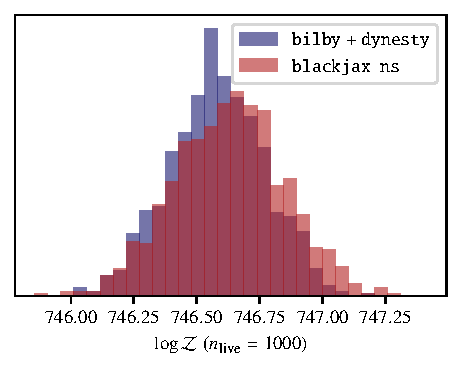
\includegraphics{figures/4s_logZ_comparison.pdf}
    \caption{Comparison of the log evidence for the 4s signal. The results are in excellent agreement, demonstrating the
    robustness of the \texttt{blackjax ns} implementation in recovering the same posteriors and evidence as the \texttt{bilby} implementation.
    This unifies parameter estimation and evidence evaluation into a single GPU-accelerated framework.}
    \label{fig:4s_logZ_comparison}
\end{figure}

\begin{figure*}
    \centering
    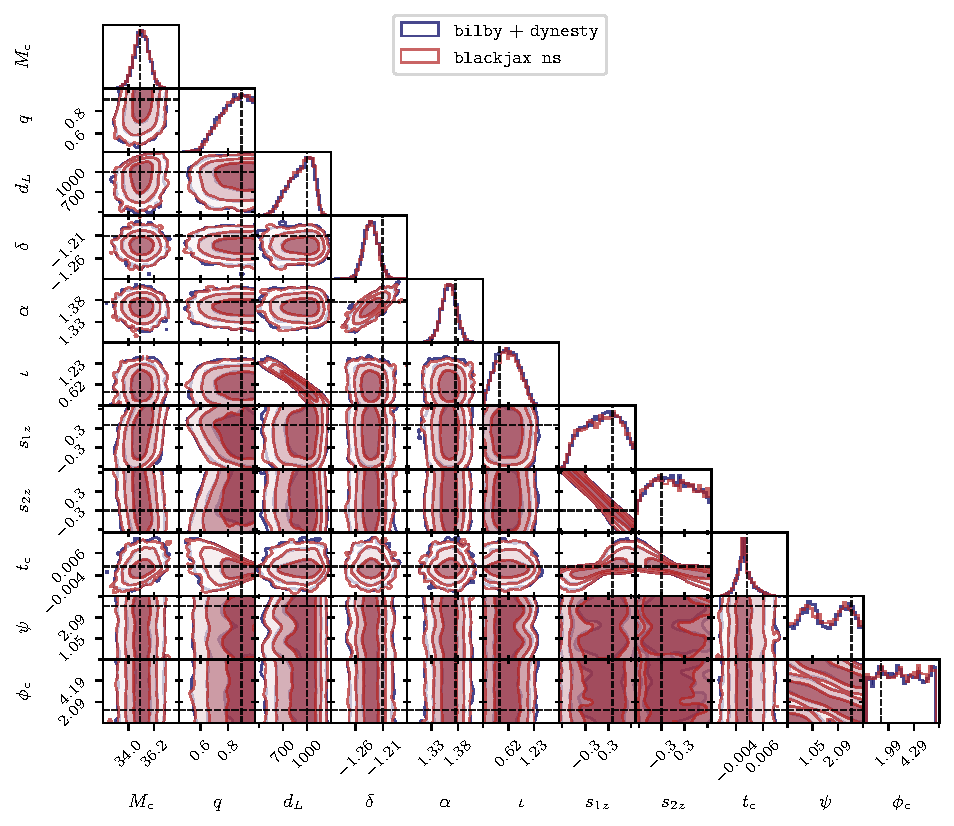
\includegraphics{figures/bilby_blackjax_comparison_4s.pdf}
    \caption{Recovered posteriors for the 4s signal. The posteriors are in agreement with each other, demonstrating that
    \texttt{blackjax ns} implementation with our custom kernel is functionally equivalent to the \texttt{bilby} + \texttt{dynesty} implementation.}
    \label{fig:4s_posteriors}
\end{figure*}


\subsection{Injection Study}

Give details of exact injections and comparison with bilby+dynesty. Write here about pp-plots?

\subsection{Real Data}

Give real data examples.

\section{Discussion}

Compare to bilby in terms of runtimes!

\section{Conclusions}

Talk about putting more waveforms on GPU. Current things we have not implemented that are available in bilby. The compatibility of using NFs with this, as we can evaluate many samples at once, meaning approaches like in nessai or PR become more efficient. 

\section*{Acknowledgements}

The Acknowledgements section is not numbered. Here you can thank helpful
colleagues, acknowledge funding agencies, telescopes and facilities used etc.
Try to keep it short.

%%%%%%%%%%%%%%%%%%%%%%%%%%%%%%%%%%%%%%%%%%%%%%%%%%
\section*{Data Availability}

 
The inclusion of a Data Availability Statement is a requirement for articles published in MNRAS. Data Availability Statements provide a standardised format for readers to understand the availability of data underlying the research results described in the article. The statement may refer to original data generated in the course of the study or to third-party data analysed in the article. The statement should describe and provide means of access, where possible, by linking to the data or providing the required accession numbers for the relevant databases or DOIs.




%%%%%%%%%%%%%%%%%%%% REFERENCES %%%%%%%%%%%%%%%%%%

% The best way to enter references is to use BibTeX:

\bibliographystyle{mnras}
\bibliography{references} % if your bibtex file is called example.bib


% Alternatively you could enter them by hand, like this:
% This method is tedious and prone to error if you have lots of references
%\begin{thebibliography}{99}
%\bibitem[\protect\citeauthoryear{Author}{2012}]{Author2012}
%Author A.~N., 2013, Journal of Improbable Astronomy, 1, 1
%\bibitem[\protect\citeauthoryear{Others}{2013}]{Others2013}
%Others S., 2012, Journal of Interesting Stuff, 17, 198
%\end{thebibliography}

%%%%%%%%%%%%%%%%%%%%%%%%%%%%%%%%%%%%%%%%%%%%%%%%%%

%%%%%%%%%%%%%%%%% APPENDICES %%%%%%%%%%%%%%%%%%%%%

\appendix

\section{Some extra material}

If you want to present additional material which would interrupt the flow of the main paper,
it can be placed in an Appendix which appears after the list of references.

%%%%%%%%%%%%%%%%%%%%%%%%%%%%%%%%%%%%%%%%%%%%%%%%%%


% Don't change these lines
\bsp	% typesetting comment
\label{lastpage}
\end{document}